\begin{frame} \frametitle{RedBlack 1}
	\begin{columns}
	
	\begin{column}{5cm}
	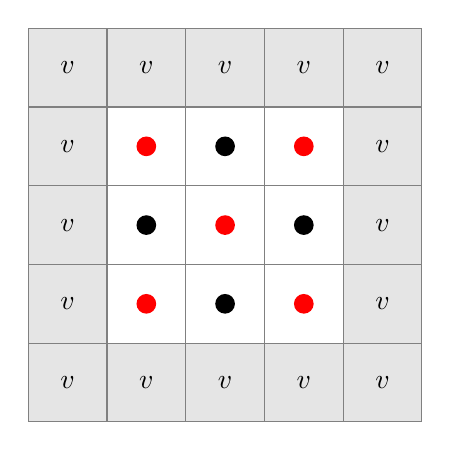
\begin{tikzpicture}
		\fill [gray!20] (-2,-2) rectangle +(1,5);
		\fill [gray!20] (2,-2) rectangle +(1,5);
		\fill [gray!20] (-2,-2) rectangle +(5,1);
		\fill [gray!20] (-2,2) rectangle +(5,1);
		\draw [step=1cm,gray] (-2,-2) grid (3,3);
		
		\fill [color=red] (.5,.5) circle [radius=.125cm];
		\fill [color=red] (-.5,-.5) circle [radius=.125cm];
		\fill [color=red] (-.5,1.5) circle [radius=.125cm];
		\fill [color=red] (1.5,1.5) circle [radius=.125cm];
		\fill [color=red] (1.5,-.5) circle [radius=.125cm];
		\fill [color=black] (-.5,.5) circle [radius=.125cm];
		\fill [color=black] (.5,1.5) circle [radius=.125cm];
		\fill [color=black] (.5,-.5) circle [radius=.125cm];
		\fill [color=black] (1.5,.5) circle [radius=.125cm];
		
		\node at (-1.5,2.5) {$v$};
		\node at (-.5,2.5) {$v$};
		\node at (.5,2.5) {$v$};
		\node at (1.5,2.5) {$v$};
		\node at (2.5,2.5) {$v$};
		\node at (2.5,1.5) {$v$};
		\node at (2.5,.5) {$v$};
		\node at (2.5,-.5) {$v$};
		\node at (2.5,-1.5) {$v$};
		\node at (1.5,-1.5) {$v$};
		\node at (.5,-1.5) {$v$};
		\node at (-.5,-1.5) {$v$};
		\node at (-1.5,-1.5) {$v$};
		\node at (-1.5,-.5) {$v$};
		\node at (-1.5,.5) {$v$};
		\node at (-1.5,1.5) {$v$};
	\end{tikzpicture}
	\end{column}
	
	\begin{column}{6cm}
	z.B. Modell f"ur eine stark vereinfachte zweidimensionale W"armeverteilung:
	\begin{itemize}
		\item Rand: Initialisierung mit Wert $v$
		\item Aktualisierung der inneren Gitterpunkte nach Rot/Schwarz-Schema
	\end{itemize}
	\end{column}
	\end{columns}
\end{frame}

\begin{frame} [fragile] \frametitle{RedBlack 2}
	\begin{columns}
	
	\begin{column}{4cm}
	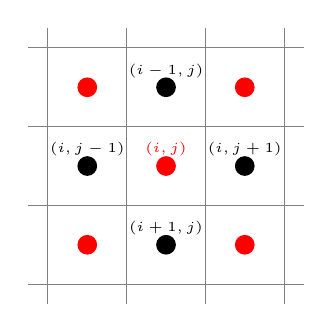
\begin{tikzpicture} [font=\tiny]
		\draw [step=1cm,gray] (-1.25,-1.25) grid (2.25,2.25);
		
		\fill [red] (.5,.5) circle [radius=.125cm] node [above] {$(i,j)$};
		\fill [red] (-.5,-.5) circle [radius=.125cm];
		\fill [red] (-.5,1.5) circle [radius=.125cm];
		\fill [red] (1.5,1.5) circle [radius=.125cm];
		\fill [red] (1.5,-.5) circle [radius=.125cm];
		\fill [black] (-.5,.5) circle [radius=.125cm] node [above] {$(i,j-1)$};
		\fill [black] (.5,1.5) circle [radius=.125cm] node [above] {$(i-1,j)$};
		\fill [black] (.5,-.5) circle [radius=.125cm] node [above] {$(i+1,j)$};
		\fill [black] (1.5,.5) circle [radius=.125cm] node [above] {$(i,j+1)$};		
	\end{tikzpicture}
	\end{column}
	
	\begin{column}{7.75cm}
		\begin{lstlisting}
		for(it=0; it<50; it++) {
		
		for(i=1; i<SIZE-1; i++)
		   for(j=1+(i%2); j<SIZE-1; j+=2)
		      m[i*SIZE+j] = ( m[(i-1)*SIZE +j] +
		                      m[(i+1)*SIZE +j] +
		                      m[ i*SIZE + j-1] +
		                      m[ i*SIZE + j+1] )/4.0;

		for(i=1; i<SIZE-1; i++)
		   for(j=1+((i+1)%2); j<SIZE-1; j+=2)
		      m[i*SIZE+j] = ( m[(i-1)*SIZE +j] +
		                      m[(i+1)*SIZE +j] +
		                      m[ i*SIZE + j-1] +
		                      m[ i*SIZE + j+1] )/4.0;
		}
		\end{lstlisting}
	\end{column}
	\end{columns}
	
	Matrix \texttt{m} der Gr"o"se \texttt{SIZE*SIZE} linear im Speicher abgelegt
\end{frame}

